\documentclass{article}

\usepackage{tikz}
\usetikzlibrary{arrows}
\usetikzlibrary{automata}
\usetikzlibrary{calc}
\usetikzlibrary{positioning}

\begin{document}

\paragraph{Fragments}

\[
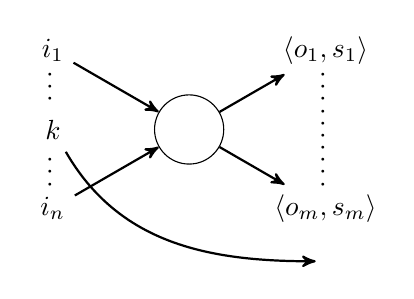
\begin{tikzpicture}

  \node [state] (A) {};

  \node (in_1) at ($(A)+(150:2cm)$) {$i_1$};
  \node (in_n) at ($(A)+(210:2cm)$) {$i_n$};
  \path (in_1) -- node [rotate=90] {\parbox{1.6cm}{\dotfill}} (in_n); 
  \node [circle,fill=white] (in_k) at ($(A)+(180:1.73cm)$) {$k$};

  \node (out_1) at ($(A)+(30:2cm)$) {$\langle o_1, s_1 \rangle$};
  \node (out_m) at ($(A)+(-30:2cm)$) {$\langle o_m, s_m \rangle$};
  \path (out_1) -- node [rotate=90] {\parbox{1.6cm}{\dotfill}} (out_m); 

  \node [below=0.25cm of out_m] (out_s) {};

  \path [draw,thick,->,>=stealth']
    (A)    edge (out_1)
    (A)    edge (out_m)
    (in_1) edge (A)
    (in_k) edge [out=-60,in=180] (out_s) 
    (in_n) edge (A);
\end{tikzpicture}
\]
On the left is the fragment's In list, on the right is the fragment's Out list. The In list is a list of vertices. The Out list is a list of vertex-insertion point pairs. $k$ is the position in the In list at which skips around this fragment should be inserted. What this means is described below.

\paragraph{Literal fragments}

\[
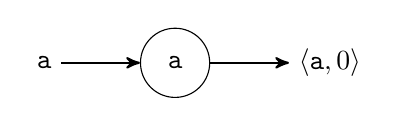
\begin{tikzpicture}

  \node [state] (A) {\texttt{a}};
  
  \node [left=1cm of A] (in) {\texttt{a}};
  \node [right=1cm of A] (out) {$\langle \texttt{a}, 0 \rangle$};

  \path [draw,thick,->,>=stealth']
    (in) edge (A)
    (A)  edge (out);
  
\end{tikzpicture}
\]
For ease of reference, we refer to the \texttt{a} vertex as \texttt{a}, though in practice it would have an index. $k = \emptyset$, which means that this fragment is not skippable. $\langle \texttt{a}, 1\rangle$ means that the next new edge leaving \texttt{a} should be inserted into vertex \texttt{a}'s edge list starting at index $0$.

\paragraph{Repetition}

\begin{center}
\begin{tabular}{cc}

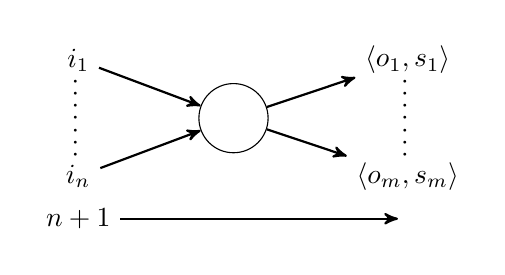
\begin{tikzpicture}
  \matrix [column sep=1cm] {
    \node (in_1) {$i_1$}; && \node (out_1) {$\langle o_1, s_1 \rangle$}; \\
    & \node [state] (A) {}; & \\
    \node (in_n) {$i_n$}; && \node (out_m) {$\langle o_m, s_m \rangle$}; \\
    \node (in_k) {$n+1$}; && \node (out_k) {}; \\
  };

  \path (in_1)  -- node [rotate=90] {\parbox{1.1cm}{\dotfill}} (in_n); 
  \path (out_1) -- node [rotate=90] {\parbox{1.1cm}{\dotfill}} (out_m); 

  \path [draw,thick,->,>=stealth']
    (in_1) edge (A)
    (in_k) edge (out_k) 
    (in_n) edge (A)
    (A)    edge (out_1)
    (A)    edge (out_m);

\end{tikzpicture}
&
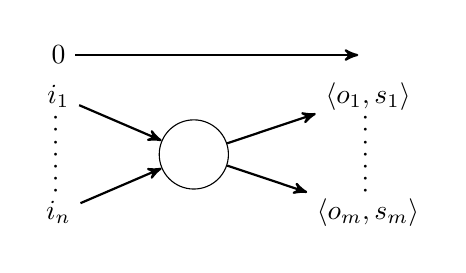
\begin{tikzpicture}
  \matrix [column sep=1cm] {
    \node (in_k) {$0$}; && \node (out_k) {}; \\
    \node (in_1) {$i_1$}; && \node (out_1) {$\langle o_1, s_1 \rangle$}; \\
    & \node [state] (A) {}; & \\
    \node (in_n) {$i_n$}; && \node (out_m) {$\langle o_m, s_m \rangle$}; \\
  };

  \path (in_1)  -- node [rotate=90] {\parbox{1.1cm}{\dotfill}} (in_n); 
  \path (out_1) -- node [rotate=90] {\parbox{1.1cm}{\dotfill}} (out_m); 

  \path [draw,thick,->,>=stealth']
    (in_1) edge (A)
    (in_k) edge (out_k) 
    (in_n) edge (A)
    (A)    edge (out_1)
    (A)    edge (out_m);

\end{tikzpicture}
\\
Greedy repetition
&
Nongreedy repetition
\end{tabular}
\end{center}

\paragraph{Grouping}

\paragraph{Concatenation}

\paragraph{Alternation}



\end{document}
